%%%%%%%%%%%%%%%%%%%%%%%%%%%%%%%%%%%%%%%%%%%%%%%%%%%%%%%%%%%%%%%%%%%%%%%%%%%%%%%
% Definici�n del tipo de documento.                                           % 
% Posibles tipos de papel: a4paper, letterpaper, legalpapper                  %
% Posibles tama�os de letra: 10pt, 11pt, 12pt                                 %
% Posibles clases de documentos: article, report, book, slides                %
%%%%%%%%%%%%%%%%%%%%%%%%%%%%%%%%%%%%%%%%%%%%%%%%%%%%%%%%%%%%%%%%%%%%%%%%%%%%%%%
\documentclass[10pt, spanish, a4paper]{article}

%%%%%%%%%%%%%%%%%%%%%%%%%%%%%%%%%%%%%%%%%%%%%%%%%%%%%%%%%%%%%%%%%%%%%%%%%%%%%%%
% Los paquetes permiten ampliar las capacidades de LaTeX.                     %
%%%%%%%%%%%%%%%%%%%%%%%%%%%%%%%%%%%%%%%%%%%%%%%%%%%%%%%%%%%%%%%%%%%%%%%%%%%%%%%
\usepackage[spanish]{babel}     % Paquete para definir el idioma usado.
\usepackage[latin1]{inputenc}   % Define la codificaci�n de caracteres 
                                % (latin1 es ISO 8859-1)
%\usepackage[T1]{fontenc}        % Agrega caracteres extendidos al font
\usepackage{t1enc}
\usepackage{palatino}           % Cambia el font por omision a Palatino
\usepackage{graphicx}           % Paquete para inclusi�n de gr�ficos.
%%%%%%%%%%%%%%%%%%%%%%%%%%%%%%%%%%%%%%%%%%%%%%%%%%%%%%%%%%%%%%%%%%%%%%%%%%%%%%%

% Modifico los margenes para tener m�s espacio por linea
\oddsidemargin 0.0in    % margen derecho
\evensidemargin 1.0in   % margen izquierdo
\textwidth 6.0in        % ancho del texto

% T��tulo principal del documento.
\title{\textbf{The Speaker (3era Entrega)}}

% Informaci�n sobre los autores.
\author{    
            Juan Manuel Barrenche, \textit{Padr�n Nro. 86.152}                 \\
            \texttt{ snipperme@gmail.com }                                     \\
            Mart��n Fern�ndez, \textit{Padr�n Nro. 88.171}                      \\
            \texttt{ tinchof@gmail.com }                                       \\
            Marcos J. Medrano, \textit{Padr�n Nro. 86.729}                     \\
            \texttt{ marcosmedrano0@gmail.com }                                \\
            Federico Valido, \textit{Padr�n Nro. 82.490}                       \\
            \texttt{ fvalido@gmail.com }                                       \\ 
                                                                               \\
            \normalsize{Grupo Nro. 11 (YES)}                                   \\
            \normalsize{Ayudante: Renzo Navas}                         	       \\
            \normalsize{1er. Cuatrimestre de 2009}                             \\
            \normalsize{75.06 Organizaci�n de Datos - Titular: Arturo Servetto}\\
            \normalsize{Facultad de Ingenier�a, Universidad de Buenos Aires}   \\
       }
\date{Domingo 24 de Mayo de 2009}


% Comienzo del documento
\begin{document}

\maketitle                % Inserta el t�tulo.
\thispagestyle{empty}     % Quita el n�mero en la primer p�gina.

% Resumen que aparece en la primera p�gina (antes de la tabla de contenidos)
\begin{abstract}
Breve descripci�n de la arquitectura a utilizar para la 3era entrega del trabajo pr�ctico del curso de \textit{75.06 Organizaci�n de Datos} de la c�tedra Servetto.\\
Se detallan las clases e interfaces principales y su interacci�n, pero no se hace referencia a la arquitectura 
utilizada en las entregas anteriores ya que el punto de contacto con la nueva funcionalidad es m�nimo.
Este documento ha sido desarrollado en \LaTeX.
\end{abstract}

\newpage

\section{The Big Picture}

La idea principal es implementar los compresores como \textbf{Serializadores}. En nuestra arquitectura actual, los 
serializadores son utilizados en todos los manejadores de archivos (VLFM, StraightFM,...) para hidratar y deshidratar
objetos. \\
Implementar los compresores de esta manera tiene la ventaja de no tener que modificar nuestra arquitectura 
actual, que actualmente est� funcionando correctamente. Simplemente se reemplazan serializadores actuales por los
nuevos serializadores que ser�n capaces de comprimir, en nuestro caso, los Documentos.

\begin{figure}[!htp]
\centering
\makebox[\textwidth]{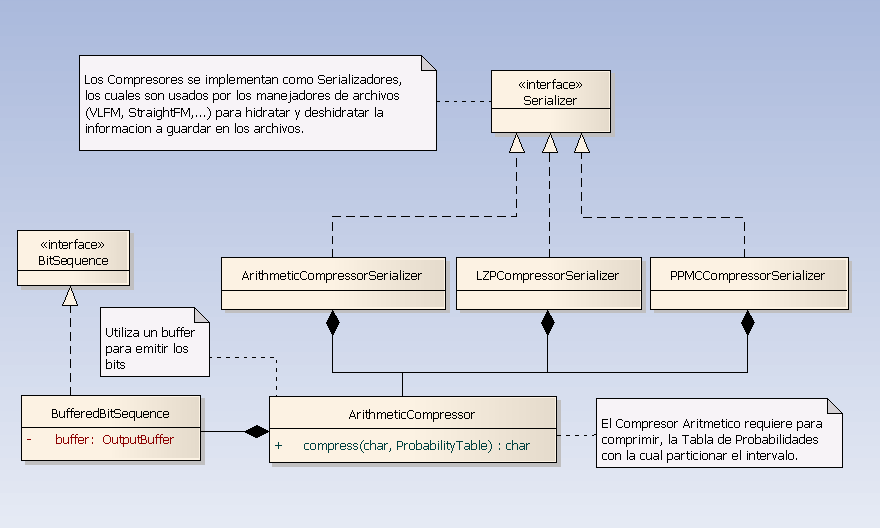
\includegraphics[scale=0.5,natwidth=20pt,natheight=10pt]{img/general.png}}
	\caption{Diagrama de clases general de la arquitectura propuesta}
\end{figure}

\section{Procesado Aritm�tico}
Todo el manejo de rangos propio del aritm�tico se concentr� en la clase \textit{ArithmeticProcessor}. La cual mantiene el estado de piso y techo y, adem�s, conoce cuando deben generarse overflows y underflows. Cada vez que se le pide procesa un �nico paso de aritm�tico (sin importar si es compresi�n o descompresi�n) con una tabla que se le pasa por par�metro y un objeto que se encarga �nicamente de decirle cual es la posici�n de la tabla de probabilidades que tiene que utilizar para quedarse como nuevo techo y piso (a este objeto se lo denomina matcher).

Esta clase es abstracta para que sus subclasificaciones definan la acci�n a realizar (comprimir o descomprimir) ya que no define ninguna interfaz p�blica. Las subclases dir�n que se hace con el resultado del proceso de la tabla. Este procesado invoca m�todos templates para hacerle saber a sus descendientes que est� ocurriendo en el process (por ejemplo, avisa cuando ocurren overflows y de que bits, etc.). 

Por ejemplo, para el caso de compresi�n, el objeto de matcher definido se basa en el caracter a comprimir y cada vez que ocurre overflow o se "limpian" los underflows acumulados emite el bit correspondiente.

En cambio, el caso de descompresi�n, toma de una entrada los bits y el matcher se basa en que valores tiene el rango para decidir en que momento debe para el proceso de la tabla. Cuando ocurren los overflow o underflows el mismo descarta de su valor actual dichos bits y solicita mas bits a la entrada. Tambi�n verifica que los bits ocultados cuando ocurri� la el underflow sean los opuestos al primer overflow que ocurra.

Esto tambi�n nos facilit� el agregado de \textit{tracers} para el aritm�tico de Orden 1 que se implement� para la prueba de este m�dulo.
\subsection{Emisi�n y lectura}
Debido a que la arquitectura de los Serializadores se basa en emisiones y lecturas de bytes (InputBuffer y OutputBuffer) pero el funcionamiento del aritm�tico emite y lee de a bits se implementaron dos clases cuyo �nico fin es adaptar esta diferencia de tama�os de manejo de datos.
La primera de ellas es el \textit{BitEmisor}, el cual toma informaci�n en bytes de un \textit{InputBuffer} y entrega bits (esto lo hace iterando sobre los bits de cada byte). 
Su contraparte es el \textit{BitReceiver}, al cual se le puede pasar datos de a bits, los junta hasta obtener un octetos que luego emite en un �nico byte en el \textit{OutputBuffer} que se le haya configurado de salida. La contra que tiene es que se le debe forzar el �ltima emisi�n por si no lleg� a obtener los 8 bits.

\begin{figure}[!htp]
\centering
\makebox[\textwidth]{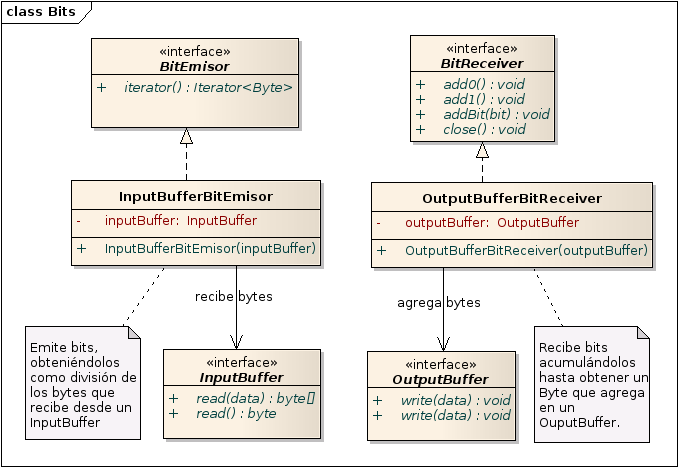
\includegraphics[scale=0.5,natwidth=20pt,natheight=10pt]{img/Bits.png}}
	\caption{Diagrama de clases para BitEmisor y BitReceiver}
\end{figure}

\subsection{Compresor y Descompresor Aritm�tico}
Como se coment� anteriormente, ambas clases extienden del proceso aritm�tico. Tratan de a un caracter por vez para que los compresores que se utilizan dentro de su forma de trabajo un aritm�tico puedan usarlo sin problema y nunca modifican la tabla de probabilidades que reciben ya que los usuarios de estas clases son los encargados de hacer mantenimiento de las mismas.

El Compresor, como se mencion� anteriormente, s�lo emite los overflow que el proceso le indique. El matcher que define se basa en el caracter a comprimir. Mientras que el descompresor toma bits de la entrada cada vez que necesita nueva informaci�n (esto ocurre cuando se detectan overflows o underflows).

\subsection{Trace del proceso aritm�tico}
Parte de los requerimientos era implementar una interfaz de consola para verificar el funcionamiento del compresor aritm�tico. Para ello se implement� un aritm�tico din�mico de Orden 1 (que maneja los contextos por medio de HashMaps) y que puede ser configurado con un PrintStream al que se le enviar�, a modo de Log, informaci�n sobre que est� sucediendo dentro del aritm�tico.

Estas capacidad de trace fue agregada en subclasificaciones de las clases de compresi�n y descompresi�n para manetener limpio el c�digo de las mismas.


\subsection{La clase Char}
La clase \textit{Char} permite tener valores fuera de los reales en un texto, es decir, el caracter \textbf{EOF}, y el 
caracter de \textbf{Escape}, que utiliza PPMC. Este �ltimo caracter tiene la particularidad que matchea con cualquier 
caracter, de manera que, en PPMC, estando en un contexto en el que no existe el caracter buscado, cuando el 
\textit{ArithmeticCompressor} verifica si el caracter matchea siempre va a encontrar que el de Escape si matchea. Es 
por esto que el compresor debe devolver el caracter de la tabla que encontr� matcheo con el recibido para que el PPMC 
pueda actuar seg�n corresponda.

\section{PPMC}

En cuanto a la arquitectura para el PPMC no hay mucho que decir, simplemente la clase PPMC se encarga de mantener las 
frecuencia de ocurrencia de los caracteres de cada contexto, las cuales se encuentran encadenadas de acuerdo a 
subniveles para facilitar la b�squeda, y de recordar cual es el contexto actual para pedirle al compresor aritm�tico 
que emita con dicha tabla de probabilidades. Cuando llama al aritm�tico arma la tabla de probabilidades excluyendo, si 
corresponde, los caracteres que otro contexto ya verific� en su tabla de frecuencias.

\begin{figure}[!htp]
\centering
\makebox[\textwidth]{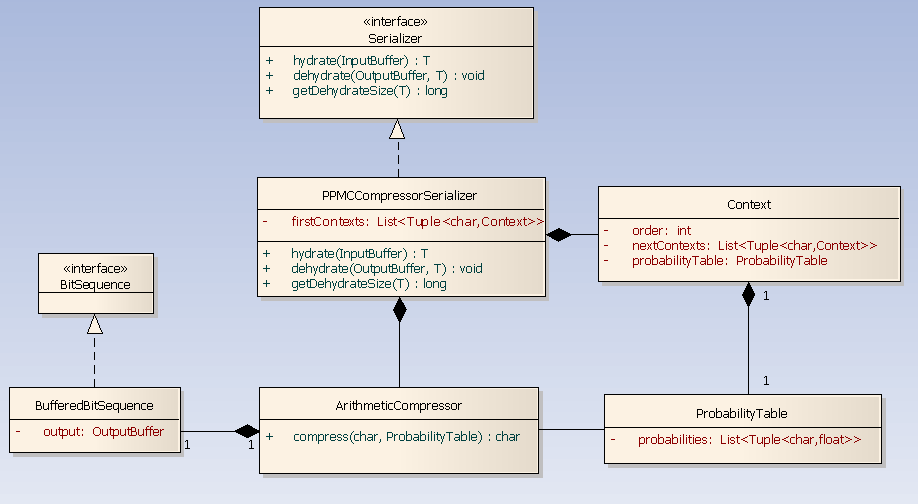
\includegraphics[scale=0.5,natwidth=20pt,natheight=10pt]{img/ppmc.png}}
\caption{Diagrama de clases de la arquitectura para PPMC}
\end{figure}

\end{document}
